\documentclass[pdf,9pt]{beamer}
\usepackage{listings,graphicx,verbatimbox,hyperref}
\usepackage{hyperref}
\usepackage{bibentry}
\usepackage[customcolors,shade]{hf-tikz}
\newcommand{\N}{\mathbb{N}}
\newcommand{\Z}{\mathbb{Z}}
\newcommand{\Q}{\mathbb{Q}}
\newcommand{\R}{\mathbb{R}}
\newcommand{\C}{\mathbb{C}}

\newcommand{\norm}[1]{\left\lVert#1\right\rVert}
\newcommand{\ceil}[1]{\lceil#1\rceil}
\newcommand{\ov}{\overline}
\newcommand{\cleq}{\preccurlyeq}
\newcommand{\cgeq}{\succcurlyeq}
\newcommand{\bdy}{\textbf{\text{Bdy}}}
\newcommand{\trace}{\text{trace}}
\newcommand{\dom}{\textbf{dom}}
\newcommand{\expec}{\mathbb{E}}
\newcommand{\bigO}{\mathcal{O}}
\newcommand{\tr}{\text{tr}}
\newcommand{\<}{\langle}
\renewcommand{\>}{\rangle}
\newcommand*\oldmacro{}%
\let\oldmacro\insertshorttitle%
% \renewcommand*\insertshorttitle{%
%   \oldmacro\hfill%
%   \insertframenumber\,/\,\inserttotalframenumber}
\DeclareMathOperator*{\argmax}{arg\,max}
\DeclareMathOperator*{\argmin}{arg\,min}

% use the below command to restart numbering in an enumeration, using alphabetics
% \setbeamertemplate{enumerate item}{(\alph{enumi})}
% \setbeamertemplate{enumerate subitem}{(\roman{enumii})}

\usetheme{Warsaw}
% \setbeamertemplate{footline}
% {
%   \leavevmode%
%   \hbox{%
%   \begin{beamercolorbox}[wd=.3\paperwidth,ht=2.25ex,dp=1ex,center]{author in head/foot}%
%     \usebeamerfont{author in head/foot}\insertshortauthor
%   \end{beamercolorbox}%
%   \begin{beamercolorbox}[wd=.7\paperwidth,ht=2.25ex,dp=1ex,center]{title in head/foot}%
%     \usebeamerfont{title in head/foot}\insertshorttitle\hspace*{3em}
%     \insertframenumber{} / \inserttotalframenumber\hspace*{0ex}
%   \end{beamercolorbox}}%
%   \vskip0pt%
% }
\setbeamertemplate{footline}[frame number]
\setbeamertemplate{navigation symbols}{}
\usepackage{biblatex}
\addbibresource{tetrad.bib}
\bibliography{tetrad}
\usepackage{caption}
\title{Feb 13 update}
%\author[cmhyett@math.arizona.edu]{Criston Hyett \inst{1}\inst{2} \and Michael Chertkov \inst{1} \and Yifeng Tian \inst{2} \and Daniel Livescu \inst{2} \and Misha Stepanov \inst{1} \and Michael Woodward \inst{1}\inst{2} \and Chris Fryer \inst{2}}

\graphicspath{{./figs/}}

\begin{document}

%%%%%%%%%%%%%%%%%%%%%%%%%%%%%%%%%%%%%%%%%%%%%%%%%%%%%%%%%%%%%%%%%%%%%%%%%%%%% 
\begin{frame}{Feb 13 Update}
  \begin{exampleblock}{Work Completed}
    \begin{itemize}
    \item Normalize $\lambda_i$ to empirical mean, and show pdf
    \item It seems that $\langle\lambda_1\rangle$ is somehow different from the estimate you have for the inverse Kolmogorov time … we need to understand the difference and if it grows with Re?
    \item We also want to see how $\langle \lambda_i\rangle / \langle \lambda_1 \rangle$ and  ratio of the second-to-first eigenvalue of strain changes with Re-number. Does it decay with Re increase?
    \item PDFs of eigenvalues of $W$ and $S$
    \end{itemize}
  \end{exampleblock}

  \begin{block}{Work In Progress}
    \begin{itemize}
    \item Generalization over Reynolds number
      \begin{itemize}
      \item Re-run training at $Re = 430$
      \end{itemize}
    \item Benefits of reduced description      
      \begin{itemize}
      \item Posteriori tests for $Re = 240,430$ - more stable?
      \end{itemize}
    \item Explanation
      \begin{itemize}
      \item Can $\lambda_{3,4,5}$ be expressed in terms of $\lambda_{1,2}$?
      \item Can we improve performance if we train with 'weaker' normalization (maybe $\tau' = 100\tau$) so that all features are of comparable size?
      \end{itemize}
    \end{itemize}
  \end{block}
  
\end{frame}
%%%%%%%%%%%%%%%%%%%%%%%%%%%%%%%%%%%%%%%%%%%%%%%%%%%%%%%%%%%%%%%%%%%%%%%%%%%%%


%%%%%%%%%%%%%%%%%%%%%%%%%%%%%%%%%%%%%%%%%%%%%%%%%%%%%%%%%%%%%%%%%%%%%%%%%%%%%
\begin{frame}{Normalize $\lambda_i$ to empirical mean, and show pdf}
  \begin{figure}
    \centering
    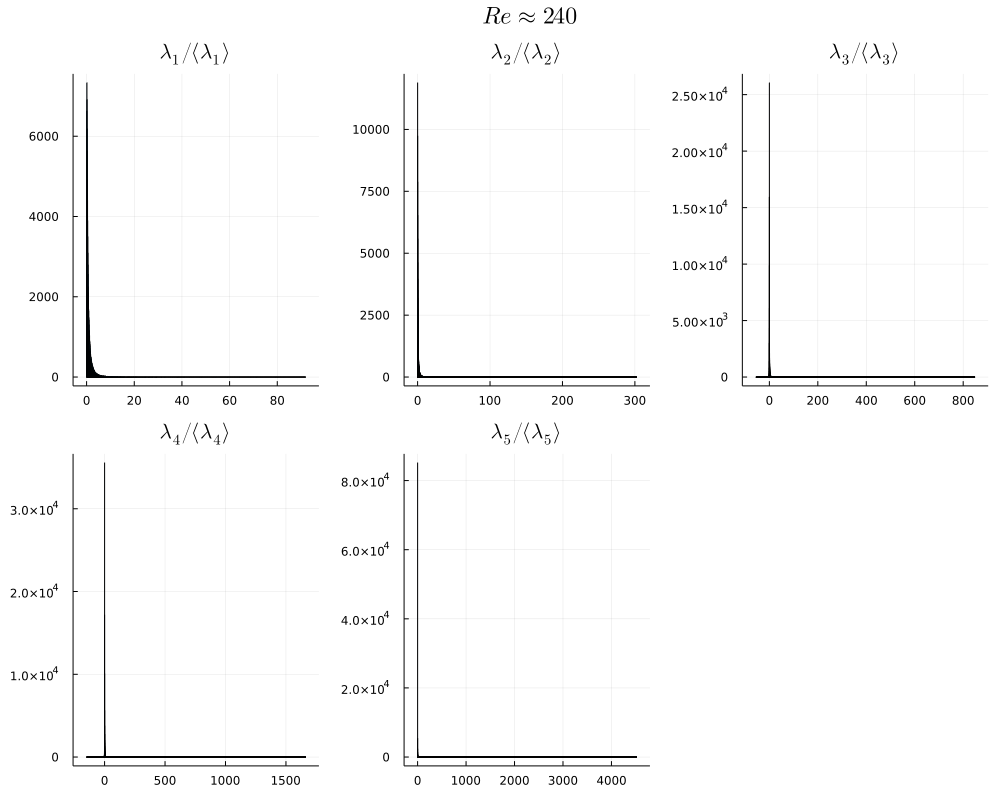
\includegraphics[width=\textwidth]{invars_250.png}
  \end{figure}
\end{frame}
%%%%%%%%%%%%%%%%%%%%%%%%%%%%%%%%%%%%%%%%%%%%%%%%%%%%%%%%%%%%%%%%%%%%%%%%%%%%%

%%%%%%%%%%%%%%%%%%%%%%%%%%%%%%%%%%%%%%%%%%%%%%%%%%%%%%%%%%%%%%%%%%%%%%%%%%%%%
\begin{frame}{Normalize $\lambda_i$ to empirical mean, and show pdf}
  \begin{figure}
    \centering
    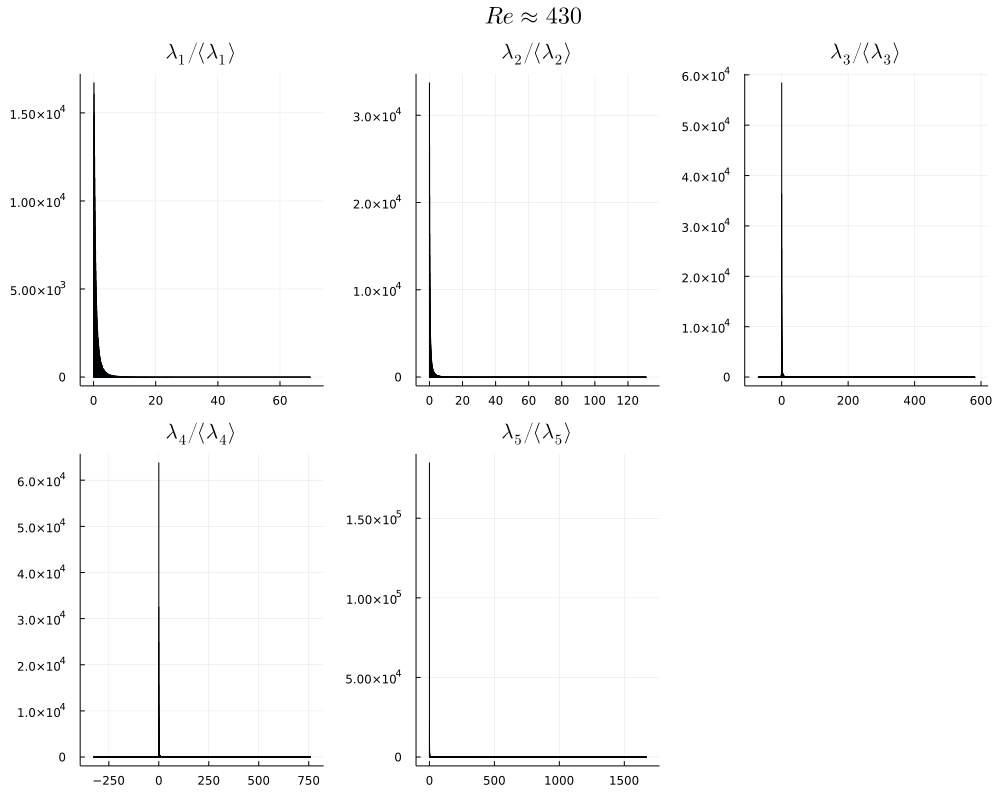
\includegraphics[width=\textwidth]{invars_450.png}
  \end{figure}
\end{frame}
%%%%%%%%%%%%%%%%%%%%%%%%%%%%%%%%%%%%%%%%%%%%%%%%%%%%%%%%%%%%%%%%%%%%%%%%%%%%%

%%%%%%%%%%%%%%%%%%%%%%%%%%%%%%%%%%%%%%%%%%%%%%%%%%%%%%%%%%%%%%%%%%%%%%%%%%%%%
\begin{frame}{Normalize $\lambda_i$ to empirical mean, and show pdf}
  \begin{figure}
    \centering
    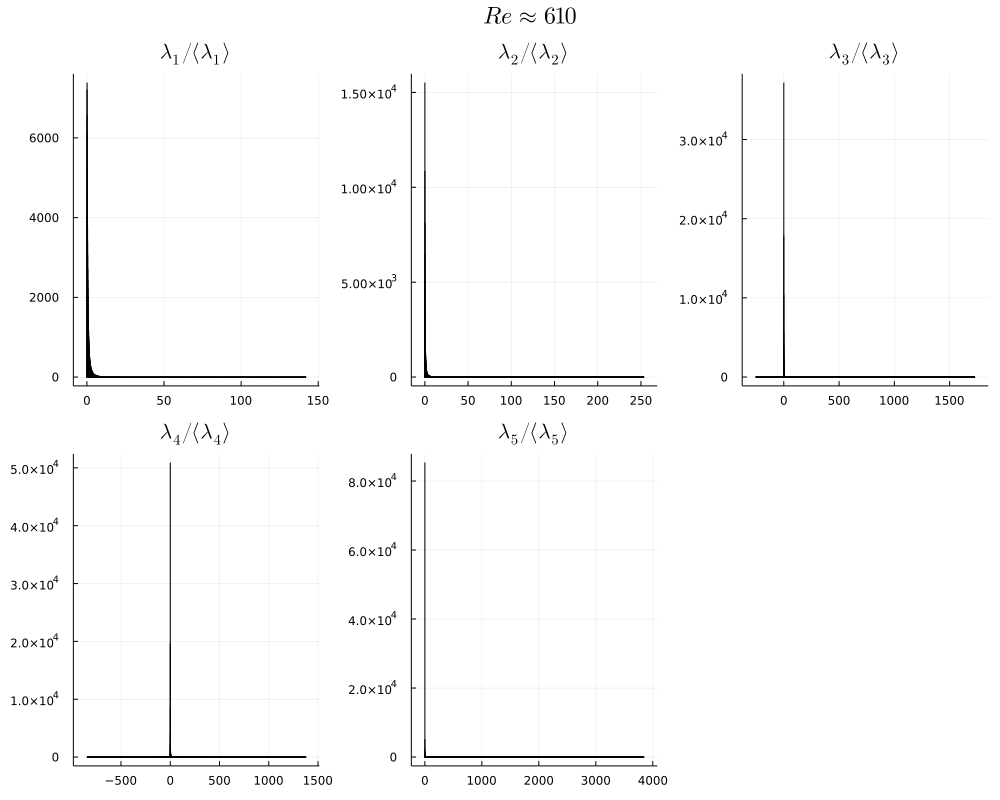
\includegraphics[width=\textwidth]{invars_650.png}
  \end{figure}
\end{frame}
%%%%%%%%%%%%%%%%%%%%%%%%%%%%%%%%%%%%%%%%%%%%%%%%%%%%%%%%%%%%%%%%%%%%%%%%%%%%%

%%%%%%%%%%%%%%%%%%%%%%%%%%%%%%%%%%%%%%%%%%%%%%%%%%%%%%%%%%%%%%%%%%%%%%%%%%%%%
\begin{frame}{Normalize $\lambda_i$ to empirical mean, and show pdf}
  \begin{figure}
    \centering
    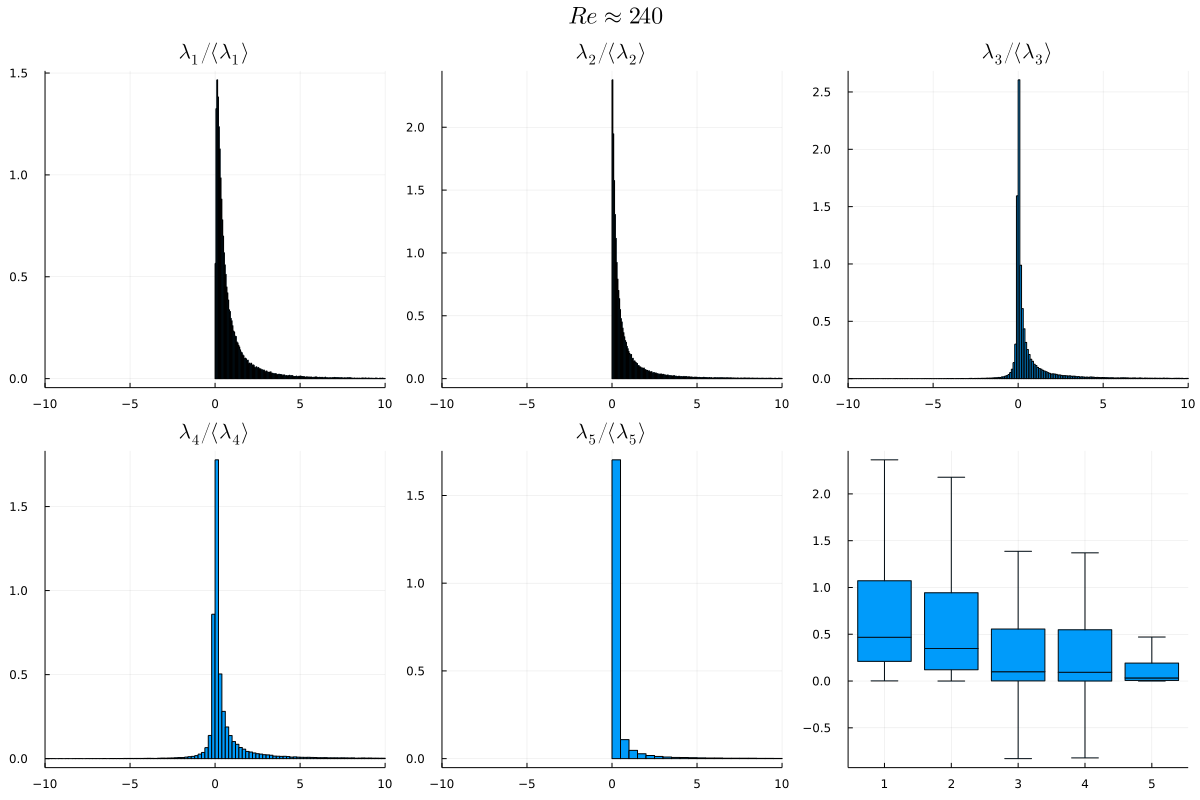
\includegraphics[width=\textwidth]{zoomedInvars_240.png}
  \end{figure}
\end{frame}
%%%%%%%%%%%%%%%%%%%%%%%%%%%%%%%%%%%%%%%%%%%%%%%%%%%%%%%%%%%%%%%%%%%%%%%%%%%%%

%%%%%%%%%%%%%%%%%%%%%%%%%%%%%%%%%%%%%%%%%%%%%%%%%%%%%%%%%%%%%%%%%%%%%%%%%%%%%
\begin{frame}{Normalize $\lambda_i$ to empirical mean, and show pdf}
  \begin{figure}
    \centering
    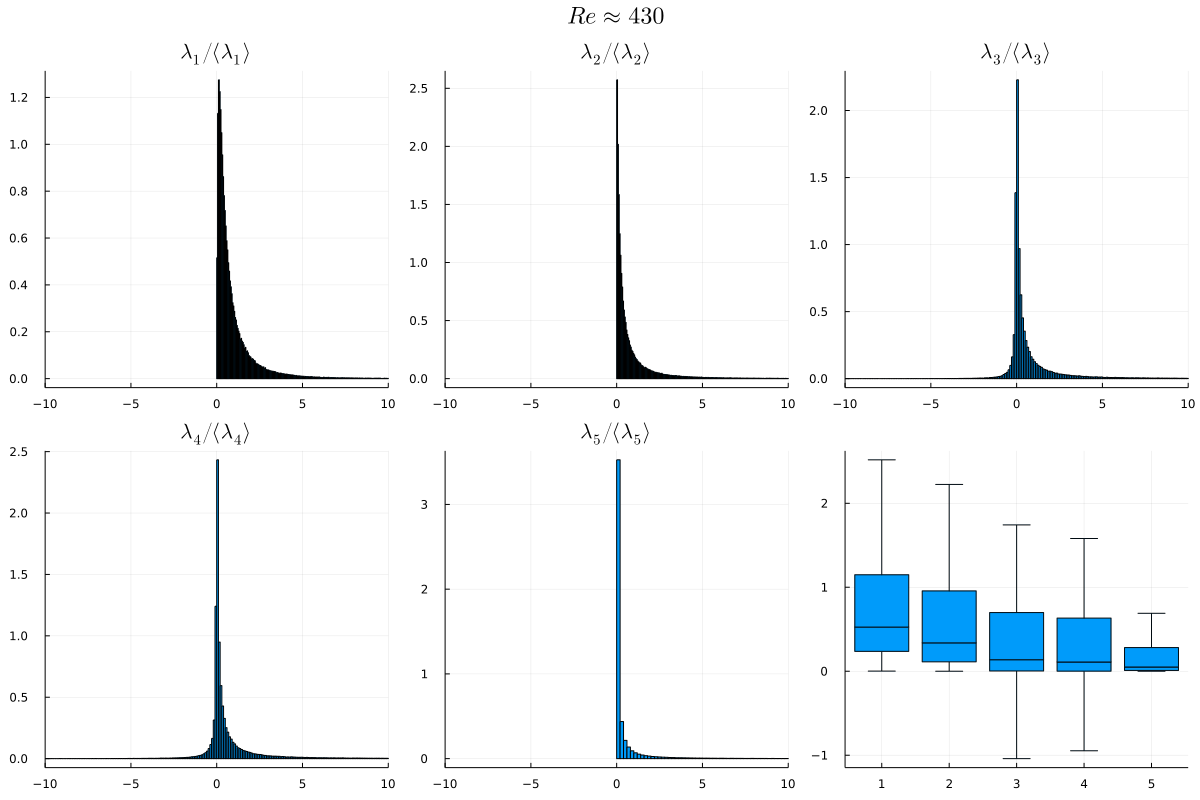
\includegraphics[width=\textwidth]{zoomedInvars_430.png}
  \end{figure}
\end{frame}
%%%%%%%%%%%%%%%%%%%%%%%%%%%%%%%%%%%%%%%%%%%%%%%%%%%%%%%%%%%%%%%%%%%%%%%%%%%%%

%%%%%%%%%%%%%%%%%%%%%%%%%%%%%%%%%%%%%%%%%%%%%%%%%%%%%%%%%%%%%%%%%%%%%%%%%%%%%
\begin{frame}{Normalize $\lambda_i$ to empirical mean, and show pdf}
  \begin{figure}
    \centering
    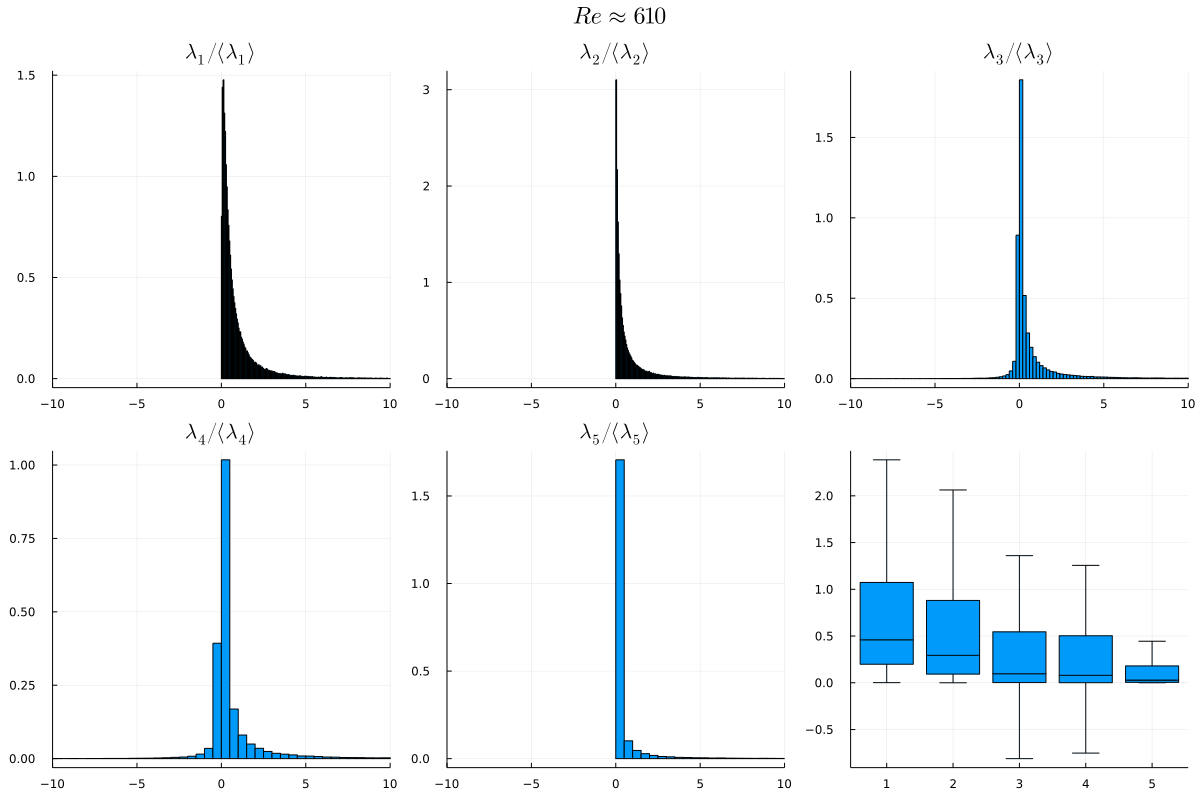
\includegraphics[width=\textwidth]{zoomedInvars_610.png}
  \end{figure}
\end{frame}
%%%%%%%%%%%%%%%%%%%%%%%%%%%%%%%%%%%%%%%%%%%%%%%%%%%%%%%%%%%%%%%%%%%%%%%%%%%%%


%%%%%%%%%%%%%%%%%%%%%%%%%%%%%%%%%%%%%%%%%%%%%%%%%%%%%%%%%%%%%%%%%%%%%%%%%%%%%
\begin{frame}{Compare $\langle \lambda_1 \rangle$ with $\tau_{Kolmogorov}^{-1}$}
  \begin{equation}
    \langle \lambda_1 \rangle = \langle \tr (S^2) \rangle
  \end{equation}
  \begin{equation}
    \tau_{Kolmogorov}^{-1} = \left\langle \norm{S^2} \right\rangle = \left\langle \sqrt{\tr(S^2)} \right\rangle
  \end{equation}
\end{frame}
%%%%%%%%%%%%%%%%%%%%%%%%%%%%%%%%%%%%%%%%%%%%%%%%%%%%%%%%%%%%%%%%%%%%%%%%%%%%%

%%%%%%%%%%%%%%%%%%%%%%%%%%%%%%%%%%%%%%%%%%%%%%%%%%%%%%%%%%%%%%%%%%%%%%%%%%%%%
\begin{frame}{$\langle \lambda_i \rangle / \langle \lambda_1 \rangle$ vs $Re$}
  \begin{figure}
    \centering
    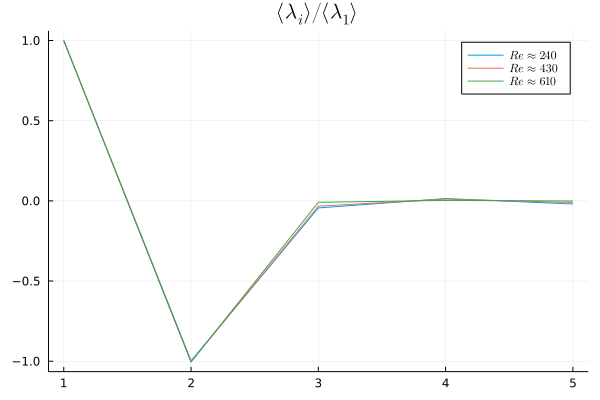
\includegraphics[width=0.5\textwidth]{invarsNormalizedToLambda1.png}%
    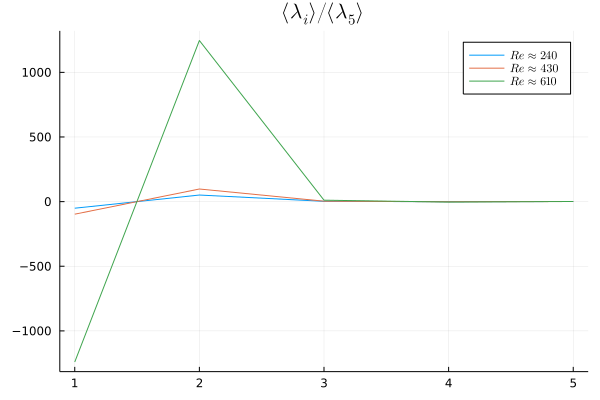
\includegraphics[width=0.5\textwidth]{invarsNormalizedToLambda5.png}
  \end{figure}
\end{frame}
%%%%%%%%%%%%%%%%%%%%%%%%%%%%%%%%%%%%%%%%%%%%%%%%%%%%%%%%%%%%%%%%%%%%%%%%%%%%%

%%%%%%%%%%%%%%%%%%%%%%%%%%%%%%%%%%%%%%%%%%%%%%%%%%%%%%%%%%%%%%%%%%%%%%%%%%%%%
\begin{frame}{Can we improve performance if we train with 'weaker' normalization (maybe $\tau' = 100\tau$) so that all features are of comparable size?}
  \begin{figure}
    \centering
    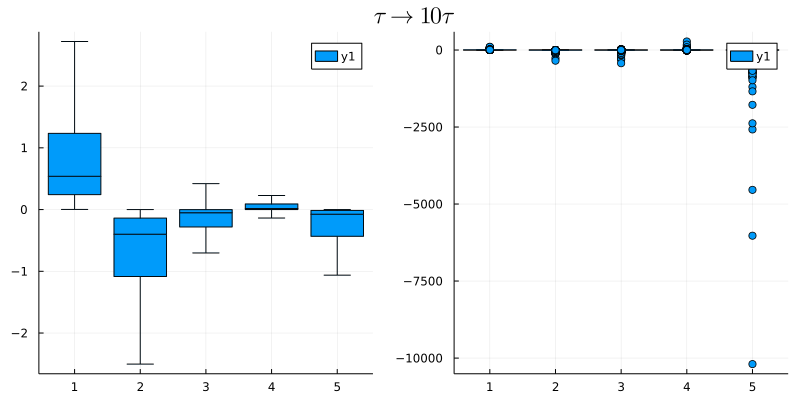
\includegraphics[width=\textwidth]{differentNormalization.png}
    \caption{$Re = 240$ data normalized with $10\tau$, plotted with and without 'outliers', points that signficantly deviate from interquartile distance. The figure shows the difficulty in normalization/nondimensionalizing as the high-order invariants have very long tails.}
  \end{figure}
\end{frame}
%%%%%%%%%%%%%%%%%%%%%%%%%%%%%%%%%%%%%%%%%%%%%%%%%%%%%%%%%%%%%%%%%%%%%%%%%%%%%

%%%%%%%%%%%%%%%%%%%%%%%%%%%%%%%%%%%%%%%%%%%%%%%%%%%%%%%%%%%%%%%%%%%%%%%%%%%%%
\begin{frame}{Re-run training at $Re \approx 430$}

\end{frame}
%%%%%%%%%%%%%%%%%%%%%%%%%%%%%%%%%%%%%%%%%%%%%%%%%%%%%%%%%%%%%%%%%%%%%%%%%%%%%

%%%%%%%%%%%%%%%%%%%%%%%%%%%%%%%%%%%%%%%%%%%%%%%%%%%%%%%%%%%%%%%%%%%%%%%%%%%%%
\begin{frame}{Re-run training with different characteristic timescale}

\end{frame}
%%%%%%%%%%%%%%%%%%%%%%%%%%%%%%%%%%%%%%%%%%%%%%%%%%%%%%%%%%%%%%%%%%%%%%%%%%%%%

%%%%%%%%%%%%%%%%%%%%%%%%%%%%%%%%%%%%%%%%%%%%%%%%%%%%%%%%%%%%%%%%%%%%%%%%%%%%%
\begin{frame}{PDFs of eigenvalues of $W$ and $S$, particularly compared to $\lambda$'s}
  \begin{figure}
    \centering
    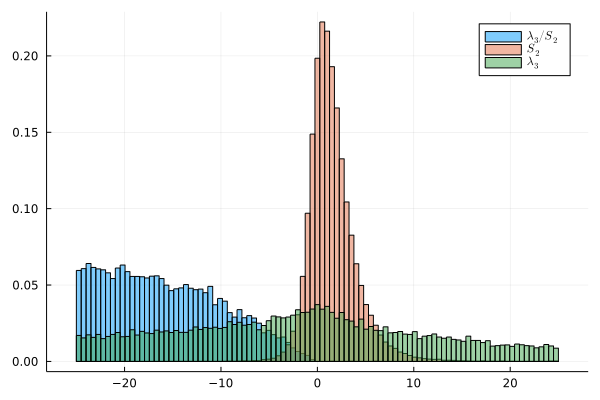
\includegraphics[width=\textwidth]{preferentialAlignment_S2_lambda3.png}
    \caption{$Re = 240$ data, showing that $\lambda_3 / S_2$ strongly prefers negative, even though neither $\lambda_3$ or $S_2$ have strong preference individually. Bug, these are not normalized.}
  \end{figure}
\end{frame}
%%%%%%%%%%%%%%%%%%%%%%%%%%%%%%%%%%%%%%%%%%%%%%%%%%%%%%%%%%%%%%%%%%%%%%%%%%%%%

\end{document}